\section{Vector Bundles}

\begin{definition}
    Let $M$ be a \underline{topological space}. A \emph{real vector bundle of rank $k$ over $M$} is a topological space $E$ together with a continuous surjection $\pi: E\onto M$ satisfying the following conditions: 
    \begin{enumerate}[label=(\alph*)]
        \item For each $p\in M$, the fiber $E_p = \pi^{-1}(p)$ over $p$ is endowed with the structure of a $k$-dimensional real vector space.
        \item For every $p\in M$, there is a neighborhood $U$ of $p$ in $M$ and a homeomorophism $\Phi:\pi^{-1}(U)\to U\times\R^k$, called a \emph{local trivialization of $E$ over $U$} satisfying the following additional conditions: 
        \begin{itemize}
            \item If $\pi_U: U\times\R^k\onto U$ is the natural projection, then $\pi_U\circ\Phi = \pi$.
            \item For each $q\in U$, the restriction of $\Phi$ to $E_q$ is a vector space isomorphism from $E_q$ to $\{q\}\times\R^k\cong\R^k$.
        \end{itemize}
    \end{enumerate}
\end{definition}

\begin{figure}[H]\label{fig:vector-bundle-illustration}
    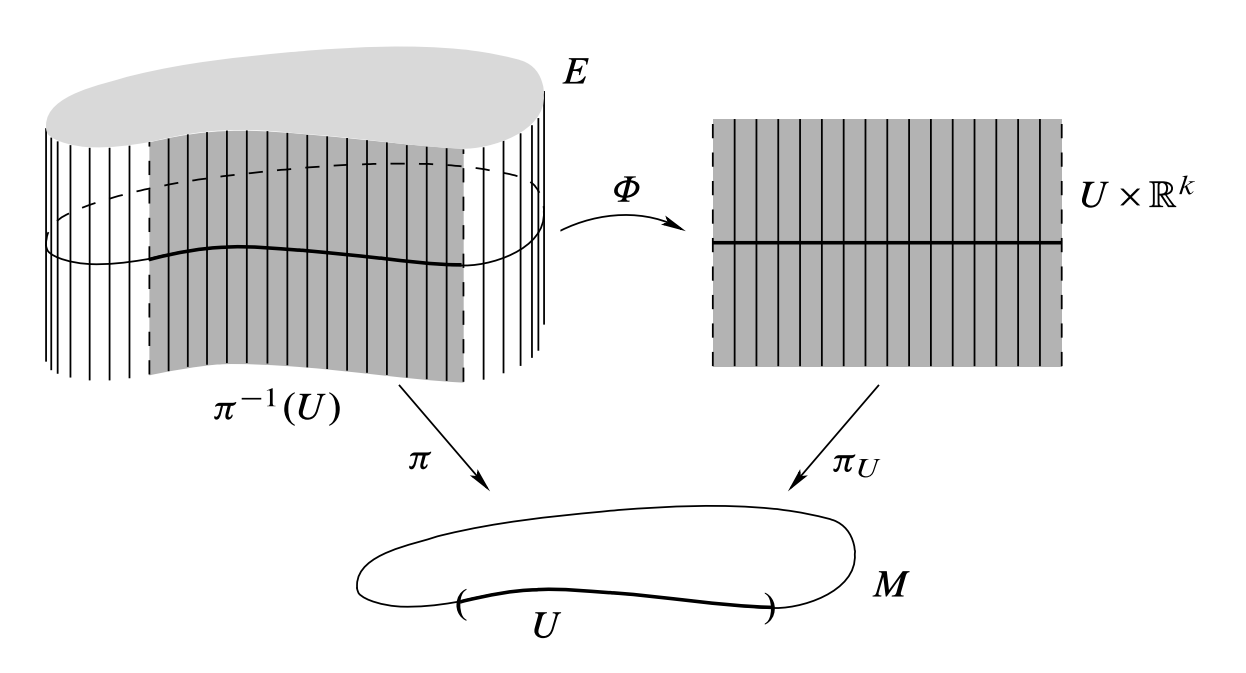
\includegraphics[width=\textwidth, height=0.3\textheight]{images/vector-bundle-illustration.png}
    \caption{A local trivialization of a vector Bundle}
\end{figure}

\begin{lemma}
    Let $\pi: E\to M$ be a smooth vector bundle of rank $k$ over $M$. Suppose $\Phi:\pi^{-1}(U)\to U\times\R^k$ and $\Psi:\pi^{-1}(V)\to V\times\R^k$ are two smooth local trivializations of $E$ with $U\cap V\ne\emptyset$. There exists a smooth map $\tau: U\cap V\to\GL(k,\R)$ such that the composition $\Phi\circ\Psi^{-1}:(U\cap V)\times\R^k\to(U\cap V)\times\R^k$ has the form 
    \begin{equation*}
        \Phi\circ\Psi^{-1}(p, v) = (p,\tau(p)v).
    \end{equation*}
\end{lemma}

\begin{lemma}[Vector Bundle Chart Lemma]\thlabel{lem:vector-bundle-chart}
    Let $M$ be a smooth manifold with or without boundary, and suppose that for each $p\in M$, there is a real vector space of fixed dimension $k$. Let $E = \coprod_{p\in M} E_p$ and let $\pi: E\to M$ be the obvious projection map. Suppose that we have 
    \begin{enumerate}[label=(\alph*)]
        \item an open cover $\{U_\alpha\}_{\alpha\in J}$ of $M$, 
        \item for each $\alpha\in J$, a bijection $\Phi_\alpha:\pi^{-1}(U_\alpha)\to U_\alpha\times\R^k$ whose restriction to each $E_p$ is a vector space isomorphism $E_p\to \{p\}\times\R^k$.
        \item for each $\alpha,\beta\in J$ with $U_\alpha\cap U_\beta\ne\emptyset$, a smooth map 
        \begin{equation*}
            \tau_{\alpha\beta}: U_\alpha\cap U_\beta\to \GL(k,\R)
        \end{equation*}
        such that the map $\Phi_\alpha\circ\Phi_{\beta}^{-1}: (U_\alpha\cap U_\beta)\times\R^k\to(U_\alpha\cap U_\beta)\times\R^k$ has the form 
        \begin{equation*}
            \Phi_\alpha\circ\Phi_\beta^{-1}(p, v) = \left(p, \tau_{\alpha\beta}(p)v\right).
        \end{equation*}
    \end{enumerate}
    Then $E$ has a unique topology and smooth structure making it into a smooth manifold with or without boundary and a smooth rank $k$ vector bundle over $M$, with $\pi: E\to M$ as a projection and $\{(U_\alpha,\Phi_\alpha)\}$ as smooth local trivializations.
\end{lemma}

\section{Local and Global Frames}

\begin{definition}[Local Section]
    Let $\pi: E\to M$ be a vector bundle and $U\subseteq M$ be open. A \emph{local section} of $E$ over $U$ is a continuous map $\sigma: U\to E$ such that $\pi\circ\sigma = \id_U$.
\end{definition}

\begin{definition}
    Let $\pi: E\to M$ be a vector bundle. If $U\subseteq M$ is an open subset, a $k$-tuple of (continuous) local sections $(\sigma_1,\dots,\sigma_k)$ of $E$ over $U$ is said to be \emph{linearly independent} if their values $(\sigma_1(p),\dots,\sigma_k(p))$ orm a linearly independent $k$-tuple in $E_p$ for each $p\in U$. Similarly, the $k$-tuple is said to \emph{span} $E$ if their values span $E_p$ for each $p\in U$.

    A \emph{local frame for $E$ over $U$} is an ordered $k$-tuple $(\sigma_1,\dots,\sigma_k)$ of linearly independent local sections over $U$ that span $E$. A local frame is called a \emph{global frame} if $U = M$.
\end{definition}

\section{The Cotangent Bundle}

\begin{definition}
    Let $V$ be a finite-dimensional vector space. A \emph{covector on $V$} is an element of the dual space $V^*$.
\end{definition}